\documentclass[%
	paper=a4,%
	DIV=calc,%
	twoside=true,%
	draft=true,%
	abstract=false]{scrartcl}

\usepackage[utf8]{inputenc}
\usepackage[english]{babel}
\usepackage{microtype}
\usepackage{graphicx}
\usepackage[load-configurations=binary]{siunitx}
	\DeclareSIUnit\Molar{\textsc{m}}
\usepackage{svn-multi}	% to add SVN-Versioning-Info
\usepackage{subfig}		% subfigures
\usepackage{booktabs}		% nice tables
\usepackage{fancyhdr}		% nice header
\usepackage{tikz}
\usepackage{pgfplots}
\usepackage[numbers,square,sort&compress]{natbib} % nice bibliography
\usepackage{scrtime}
\usepackage[version=3]{mhchem}
\usepackage{setspace}
	%\doublespacing
	%\onehalfspacing
\usepackage{lineno}
	%\linenumbers\modulolinenumbers[2]
\usepackage{lastpage}	
\usepackage[]{todonotes} 		                % [disable]
\usepackage[backref]{hyperref} 	% backref generates link from references back to text
 
% Subversion Information
\svnidlong
{$HeadURL$}
{$LastChangedDate$}
{$LastChangedRevision$}
{$LastChangedBy$}
\svnid{$Id$} 
 
\pagestyle{fancy}
\fancyfoot{}
\fancyfoot[OR]{\tiny \href{\svnkw{HeadURL}}{Rev. \svnkw{LastChangedRevision}}, commited on \svnkw{LastChangedDate} --- Page \thepage\ of \pageref{LastPage}}
\fancyfoot[EL]{\tiny Page \thepage\ of \pageref{LastPage} --- \href{\svnkw{HeadURL}}{Revision \svnkw{LastChangedRevision}}, committed on \svnkw{LastChangedDate}}
 
\newcommand{\imsize}{\linewidth}

\newcommand{\footremember}[2]{\footnote{#2}\newcounter{#1}\setcounter{#1}{\value{footnote}}}
\newcommand{\footrecall}[1]{\footnotemark[\value{#1}]}
 
\title{Acinar growth over lung development}
%\subtitle{Revision \svnkw{LastChangedRevision} | \today, \thistime}
\author{%
	David Haberthür\footremember{ana}{Institute of Anatomy, University of Bern, Switzerland}%
	\and Marco Stampanoni\footremember{psi}{Swiss Light Source, Paul Scherrer Institut, Villigen, Switzerland}\footremember{eth}{Institute for Biomedical Engineering, Swiss Federal Institute of Technology and University of Zürich, Switzerland}%
	\and Johannes C. Schittny\footrecall{ana}%
	}
\date{\today}

\begin{document}
\maketitle

\begin{abstract}
Here be the Abstract\ldots
\end{abstract}

\section{Introduction}\label{sec:Introduction}
The pulmonary acinus (gas-exchange area which is ventilated by one purely conducting airway) represents the functional unit of the lung parenchyma. Due a restricted availability of high resolution three-dimensional imaging methods the knowledge about the development of the pulmonary acini is limited. Using synchrotron radiation based tomographic microscopy \cite{Haberthuer2010a} we developed a method to evaluate the volume of single acini throughout postnatal lung development.

\begin{itemize}
	\item Gas exchange region of the terminal airway space
	\begin{itemize}
		\item Functional Lung unit $\rightarrow$ Acinus
		\item Expanding size
	\end{itemize}
	\item Prior Models
	\begin{itemize}
		\item Alveolarization
		\item Late Alveolarization
		\item Microvascular Maturation~\cite{Mund2008}
	\end{itemize}
       	\item Visualization of rat lung acini over the postnatal lung development $\rightarrow$ acini seem to grow to a greater extent than expected.
	\item SRXTM
	\begin{itemize}
		\item Classic SRXTM
		\item WF-SRXTM~\cite{Haberthuer2010}
	\end{itemize}
\end{itemize}

\section{Materials \& Methods}\label{sec:MM}
\subsection{Rat lung samples}
Rat lung samples, prepared according to \cite{Tschanz2002,Luyet2002} were used as test objects. Briefly, lungs of Sprague-Dawley rats were filled with \SI{2.5}{\percent} glutaraldehyde (\cf{CH2(CH2CHO)2}) in \SI{0.03}{\Molar} potassium-phosphate buffer (pH 7.4) by instillation via tracheotomy at a constant pressure of \SI{20}{\centi\meter} water column. In order to prevent recoiling of the lung, this pressure was maintained during glutaraldehyde-fixation for a minimum of two hours. Subsequently, the lungs were dissected free and immersed in toto in the same fixative at a temperature of \SI{4}{\celsius} for at least \SI{24}{\hour}.

The samples were postfixed with \SI{1}{\percent} osmium tetroxide (\cf{OsO4}) and stained with \SI{4}{\percent} uranyl nitrate (\cf{UO2(NO3)2}) to increase the x-ray absorption contrast, dehydrated in a graded series of ethanol and embedded in paraffin using Histoclear (Merck KGaA, Darmstadt, Germany) as an intermedium. The lung samples were mounted onto standard scanning electron microscopy sample holders (PLANO GmbH, Wetzlar, Germany) using paraffin~\cite{Tsuda2008}.

The handling of animals before and during the experiments, as well as the experiments themselves, were approved and supervised by the Swiss Agency for the Environment, Forests and Landscape and the Veterinary Service of the Canton of Bern, Switzerland.

\subsection{Tomographic data acquisition}
The experiments were performed at the TOMCAT beamline at the Swiss Light Source, Paul Scherrer Institut, Villigen, Switzerland~\cite{Stampanoni2006a}. The samples were scanned at \SI{12.6}{\kilo\electronvolt}. After penetration through the sample, the x-rays were converted into visible light by a YAG:Ce scintillator (\SI{18}{\micro\meter} thickness, Crismatec Saint-Gobain, Nemours, France). Projections were magnified by diffraction limited microscope optics (10\(\times\) magnification) and digitized by a high-resolution 2048\(\times\)2048 pixel CCD camera (pco.2000, PCO AG, Kelheim, Germany) with \SI{14}{\bit} dynamic range. The detector was operated in 2\(\times\)2 binning mode. As a result, the pixel size was \SI{1.48}{\micro\meter} and the exposure time was \SI{175}{\milli\second}\todo{already mention Wide-Field Scanning here?}.

To study the alveolar septa, a resolution in the order of one micron is required. Since we selectively wanted to choose an alveolus/multiple alveoli, a large sample volume had to be scanned. Usually, a large field of view resulting in a large sample volume can only be acquired with low magnification and vice-versa. Thus, the full volume of our samples would not have fit inside the field of view of the TOMCAT beamline at the chosen optical properties (\(1.52\times1.52\times\)\SI{1.52}{\milli\meter}).

To enhance the field of view of the TOMCAT beamline at the chosen optical configuration, we obtained tomographic datasets using a so called wide field scan~\cite{Haberthuer2010}. Briefly, several partial scans with an optimized amount of projections spanning an enlarged field of view have been independently acquired. Prior to reconstructing the tomographic dataset, these projections have been merged to one large projection spanning the desired field of view. With this approach we increased the available field of view at TOMCAT three-fold, while keeping the voxel size and reconstruction quality on the desired level and avoiding the aforementioned trade-off between voxel size and sample volume.

\subsection{Visualization and Extraction of Acini}
The tomographic datasets of the sample three-dimensionally analyzed and visualized using MeVisLab (Version 2.1 (2010-07-26 Release), MeVis Medical Solutions AG and Fraunhofer MEVIS - Institute for Medical Image Computing, Bremen, Germany). The tomograhic dateset was loaded, processed and visualized\todo{Write exact details of processing network}. Airway segments were extracted using a threshold interval based region growing algorithm~\cite{Zucker1976}. A seed point for the region growing algorithm was manually defined inside the terminal broncioloe/alveolar duct on one of the most proximal slices. The segmented airways have been visualized and cropped to a promising region of interest and exported as DICOM-file to facilitate further processing using ImageJ~\cite{Abramoff2004} and the Stepanizer~\cite{Tschanz2010}.

\begin{itemize}
	\item Extraction of Acinus
	\item Manhole Covers
	\begin{itemize}
		\item Morphological Criteria $\rightarrow$ Detection of ``Entrance Point'' into Acinus
		\item Threshold based, seeded Region Growing
		\item Pixel Volume counting
	\end{itemize}
	\item Data to measure:
	\begin{itemize}
		\item Acinar volume
		\item Acinar surface
		\item Number of alveoli
		\item Mean alveolar volume
		\item Total alveolar volume
		\item Total ductal volume
	\end{itemize}
\end{itemize}

\section{Results}\label{sec:Results}
For each day and sample we extracted multiple acini with the \emph{Manhole Cover}-method. The volumes of the extracted acini are shown in \autoref{fig:plot}.

\begin{figure}
	\centering
	\begin{tikzpicture}
		\pgfplotsset{every axis plot/.append style={semitransparent,only marks}}
		\begin{semilogyaxis}[
			xlabel=Acinus,
			ylabel=	{Volume [\si{\micro\litre}]},
			legend pos=outer north east,
			]
			\addplot
				table [x=Segment,y=Volume] {plots/R108C04.txt};
			\addplot
				table [x=Segment,y=Volume] {plots/R108C10.txt};
			\addplot
				table [x=Segment,y=Volume] {plots/R108C21.txt};
			\addplot
				table [x=Segment,y=Volume] {plots/R108C36.txt};
			\addplot
				table [x=Segment,y=Volume] {plots/R108C60.txt};
			\legend{%
				Day 04,%
				Day 10,%
				Day 21,%
				Day 36,%
				Day 60}		
		\end{semilogyaxis}
	\end{tikzpicture}
	\caption{Volumes of the extracted acini}
	\label{fig:plot}
\end{figure}

\begin{figure}
	\centering
	\pgfplotsset{width=.5\linewidth}
	\subfloat[Mean acinar volumes]{% !TEX root = ../acinus.tex

% \documentclass{article}
% \usepackage{tikz,pgfplots}
% \usepackage{siunitx}
% \usepackage[graphics,tightpage,active]{preview}
% \PreviewEnvironment{tikzpicture}
% \newcommand{\imsize}{\linewidth}
% \newlength\imagewidth           % needed for scalebars
% \newlength\imagescale           % ditto
% \begin{document}%
%%%%%%%%%%%%%%%%%%%%%%%%%%%%%%%%%%%%%%%%
	\begin{tikzpicture}
		\begin{axis}[%
			legend pos=south east,%
			scale only axis,%
			%ultra thick,%
			xlabel={Days},%
			ylabel={Volume [\si{\micro\litre}]},%
			xlabel near ticks,%
			ylabel near ticks,%
			xtick = data,%
			ytick = {0,0.02,...,0.11},%
			%ymajorgrids=true%
			]
			\addplot [blue,%
				mark=*,%
				semitransparent,%
				error bars/.cd,y dir=both,y explicit]
				coordinates {
 					(4,0.002595) +- (0.000308,0.000308)
					(10,0.012600) +- (0.001271,0.001271)
					(21,0.05602) +- (0.005973,0.005973)
					(36,0.084727) +- (0.006036,0.006036)
					(60,0.086460) +- (0.007447,0.007447)};
			\legend{Acini}
		\end{axis}
		\end{tikzpicture}
%%%%%%%%%%%%%%%%%%%%%%%%%%%%%%%%%%%%%%%%
% \end{document}
%Day	average	standard deviation	standard error of mean
%4	0.305	0.035	0.015
%10	0.508	0.048	0.022
%21	1.048	0.092	0.041
%36	2.062	0.141	0.063
%60	2.964	0.194	0.087}\\%
	\subfloat[Mean right lower lung lobe (RLL) volumes]{% !TEX root = ../acinus.tex

% \documentclass{article}
% \usepackage{tikz,pgfplots}
% \usepackage{siunitx}
% \usepackage[graphics,tightpage,active]{preview}
% \PreviewEnvironment{tikzpicture}
% \newcommand{\imsize}{\linewidth}
% \newlength\imagewidth           % needed for scalebars
% \newlength\imagescale           % ditto
% \begin{document}%
%%%%%%%%%%%%%%%%%%%%%%%%%%%%%%%%%%%%%%%%
	\begin{tikzpicture}
		%\tikzset{every mark/.append style={scale=4}}
		%\pgfplotsset{every axis legend/.append style={at={(0.8,0.08)},anchor=base}}
		\begin{axis}[%
			legend pos=south east,%
			scale only axis,%		
			%ultra thick,%
			xlabel={Days},%
			ylabel={Volume [\si{\centi\meter\cubed}]},%
			xlabel near ticks,%
			ylabel near ticks,%
			xtick = data,%
			%ytick = {0,5,...,35},%
			%ymajorgrids=true%
			]
			\addplot [red,%
				mark=square*,%
				semitransparent,%
				error bars/.cd,y dir=both,y explicit]
				coordinates {
 					(4,0.305) +- (0.015,0.015)
					(10,0.508) +- (0.022,0.022)
					(21,1.048) +- (0.041,0.041)
					(36,2.062) +- (0.063,0.063)
					(60,2.964) +- (0.087,0.087)};
		\legend{RLL}
		\end{axis}
		\end{tikzpicture}
%%%%%%%%%%%%%%%%%%%%%%%%%%%%%%%%%%%%%%%%
% \end{document}
%Day	average	standard deviation	standard error of mean
%4	0.305	0.035	0.015
%10	0.508	0.048	0.022
%21	1.048	0.092	0.041
%36	2.062	0.141	0.063
%60	2.964	0.194	0.087}\\%
	\subfloat[Volume increase based on day 4]{% !TEX root = ../acinus.tex

% \documentclass{article}
% \usepackage{tikz,pgfplots}
% \usepackage{siunitx}
% \usepackage[graphics,tightpage,active]{preview}
% \PreviewEnvironment{tikzpicture}
% \newcommand{\imsize}{\linewidth}
% \newlength\imagewidth           % needed for scalebars
% \newlength\imagescale           % ditto
% \begin{document}%
%%%%%%%%%%%%%%%%%%%%%%%%%%%%%%%%%%%%%%%%
	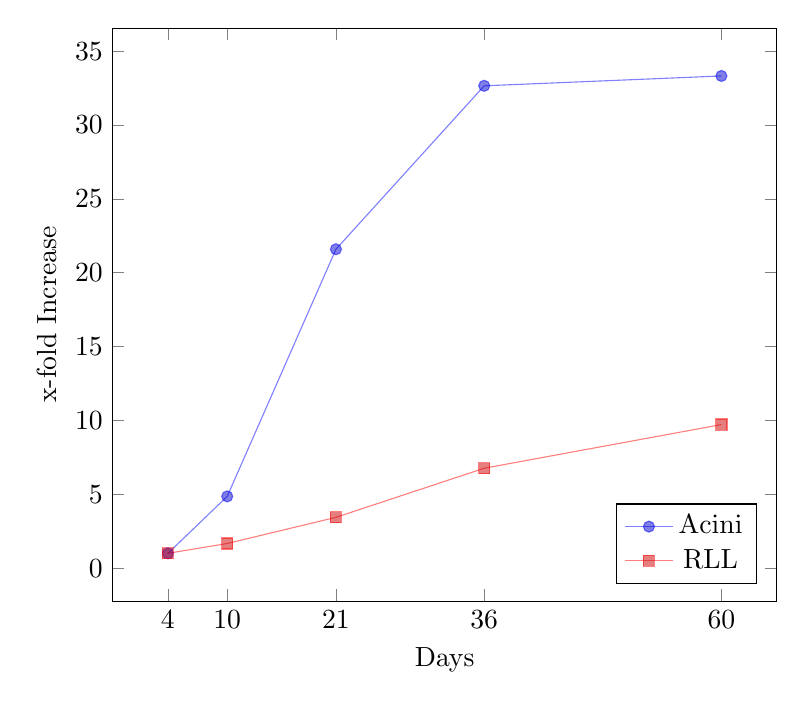
\begin{tikzpicture}
		\begin{axis}[%
			legend pos=south east,%
			scale only axis,%		
			%ultra thick,%
			xlabel={Days},%
			ylabel={x-fold Increase},%
			xlabel near ticks,%
			ylabel near ticks,%
			xtick = data,%
			ytick = {0,5,...,35},%
			%ymajorgrids=true%
			]
		\addplot+[semitransparent]
			coordinates{
		 		(4,1)
				(10,4.85549)
				(21,21.58767)
				(36,32.65010)
				(60,33.31792)
		};
		\label{plot:acini}
		\addplot+[semitransparent]
			coordinates{
				(4,1)
				(10,1.666)
				(21,3.436)
				(36,6.761)
				(60,9.718)
		};
		\label{plot:rul}
		\legend{Acini,RLL}
		\end{axis}
		\end{tikzpicture}
%%%%%%%%%%%%%%%%%%%%%%%%%%%%%%%%%%%%%%%%
% \end{document}}%
	\caption{Plot of increase in Volume for both Acini (\ref{plot:acini}) and right lower lung lobe (RLL, \ref{plot:rul}). While the volume of the right lower lung lobe increases approximately 10-fold over the first 2 months after birth, we see an approximately 33-fold increase in mean volume for the extracted acini from day \numrange{4}{60}.}
	\label{plot}
\end{figure}

We observed an approximately thirty-three-fold increase of the mean acinar volume during the postnatal lung development from days \numrange{4}{60} (33.25-fold, from \SIrange{0.00260}{0.08646}{\micro\litre}). During the same period the volume of the right lower lung lobe increases only approximately ten-fold (9.72-fold, from \SIrange{0.305}{2.964}{\centi\metre\cubed}, see \cite{Tschanz2003}), which results in an acinar growth 3.4 times larger than the right lower lung lobe volume.

\section{Discussion}\label{sec:Discussion}
We hypothesize that this large increase of the acinar volume can only be achieved by a conversion of the \numrange{2}{4} most distal purely conducting airways into alveolar ducts between birth and adulthood. As a consequence \numrange{4}{16} small acini have to be merged to a larger one. We expect that the increased complexity of the adult acini influences both ventilation and particle deposition.

\section{Acknowledgments}
\begin{itemize}
	\item Xris, Fede, Bernd
	\item Mohammed
	\item Sebastien? Or is he also on the author list?
	\item SNF
\end{itemize}
\bibliographystyle{unsrtnat}
\bibliography{../references}
 
\end{document}